\documentclass[12pt,a4paper]{article}\usepackage[]{graphicx}\usepackage[]{color}
%% maxwidth is the original width if it is less than linewidth
%% otherwise use linewidth (to make sure the graphics do not exceed the margin)
\makeatletter
\def\maxwidth{ %
  \ifdim\Gin@nat@width>\linewidth
    \linewidth
  \else
    \Gin@nat@width
  \fi
}
\makeatother

\definecolor{fgcolor}{rgb}{0.345, 0.345, 0.345}
\newcommand{\hlnum}[1]{\textcolor[rgb]{0.686,0.059,0.569}{#1}}%
\newcommand{\hlstr}[1]{\textcolor[rgb]{0.192,0.494,0.8}{#1}}%
\newcommand{\hlcom}[1]{\textcolor[rgb]{0.678,0.584,0.686}{\textit{#1}}}%
\newcommand{\hlopt}[1]{\textcolor[rgb]{0,0,0}{#1}}%
\newcommand{\hlstd}[1]{\textcolor[rgb]{0.345,0.345,0.345}{#1}}%
\newcommand{\hlkwa}[1]{\textcolor[rgb]{0.161,0.373,0.58}{\textbf{#1}}}%
\newcommand{\hlkwb}[1]{\textcolor[rgb]{0.69,0.353,0.396}{#1}}%
\newcommand{\hlkwc}[1]{\textcolor[rgb]{0.333,0.667,0.333}{#1}}%
\newcommand{\hlkwd}[1]{\textcolor[rgb]{0.737,0.353,0.396}{\textbf{#1}}}%
\let\hlipl\hlkwb

\usepackage{framed}
\makeatletter
\newenvironment{kframe}{%
 \def\at@end@of@kframe{}%
 \ifinner\ifhmode%
  \def\at@end@of@kframe{\end{minipage}}%
  \begin{minipage}{\columnwidth}%
 \fi\fi%
 \def\FrameCommand##1{\hskip\@totalleftmargin \hskip-\fboxsep
 \colorbox{shadecolor}{##1}\hskip-\fboxsep
     % There is no \\@totalrightmargin, so:
     \hskip-\linewidth \hskip-\@totalleftmargin \hskip\columnwidth}%
 \MakeFramed {\advance\hsize-\width
   \@totalleftmargin\z@ \linewidth\hsize
   \@setminipage}}%
 {\par\unskip\endMakeFramed%
 \at@end@of@kframe}
\makeatother

\definecolor{shadecolor}{rgb}{.97, .97, .97}
\definecolor{messagecolor}{rgb}{0, 0, 0}
\definecolor{warningcolor}{rgb}{1, 0, 1}
\definecolor{errorcolor}{rgb}{1, 0, 0}
\newenvironment{knitrout}{}{} % an empty environment to be redefined in TeX

\usepackage{alltt}

\usepackage{times}
\usepackage{durhampaper}

\usepackage{booktabs}
\usepackage[table]{xcolor}
\usepackage{tikz}
\usepackage{lastpage}%page 1 of \lastpage
\usepackage{float}
\usepackage{flafter}
\usepackage[british]{babel}%hypenation and spelling and stuff
\usepackage{fancyhdr}
\usepackage{subcaption}
\usepackage[section]{placeins}
\usepackage{natbib}
\usepackage{wrapfig}
\usepackage{enumitem}
\usepackage{tcolorbox}
\usepackage[all]{nowidow}


%packages to load last
\usepackage[hyphens, spaces]{url}%allow URLS
\usepackage{varioref}%Automatic page references
\usepackage[colorlinks, allcolors=blue, breaklinks]{hyperref}%Automatic reference links
\usepackage[all]{hypcap}
\usepackage[capitalise, nameinlink]{cleveref}%Automatic reference typing
\crefname{subsection}{subsection}{subsections}

\renewcommand{\harvardurl}[1]{\textbf{URL:} \url{#1}}
%\citationmode{abbr}
\bibliographystyle{agsm}

\title{Tailoring Horror Games with Biosignals}
\author{} % leave; your name goes into \student{}
\student{S.H. Lowes}
\supervisor{M.J.R. Bordewich}
\degree{BSc Computer Science}

\date{}

\setenumerate{noitemsep}

\pagestyle{fancy}
\pagenumbering{arabic}
\rhead{\small Steven Lowes}

\makeatletter
\lhead{\small \@title}
\makeatother

\lfoot{3rd May 2019}
\cfoot{Page \thepage\ of \pageref{LastPage}}

\setlength{\headheight}{14pt} 

\renewcommand{\bibsection}{}
\IfFileExists{upquote.sty}{\usepackage{upquote}}{}
\begin{document}





\maketitle
\begin{abstract}
%These instructions give you guidelines for preparing the final paper.  DO NOT change any settings, such as margins and font sizes.  Just use this as a template and modify the contents into your final paper.  Do not cite references in the abstract.

%The abstract must be a Structured Abstract with the headings {\bf Context/Background}, {\bf Aims}, {\bf Method}, {\bf Results}, and {\bf Conclusions}.  This section should not be longer than half of a page, and having no more than one or two sentences under each heading is advised.

\textbf{Context/Background}
The horror genre has consistently been one of the most popular genres of video game, thrilling players by allowing them to experience fear in a safe environment.
However, each person reacts differently to scares and the one-size-fits-all experience can prove restrictive.
Some experiments have attempted to use  to control the scares in horror games, but all have shown significant flaws in their approach or choice of sensor.

\textbf{Aims}
This project aims to answer the following research question: \emph{Can biosignals be used to tailor the timing of scares in a horror game to improve the user experience?}
The user experience will be measured in terms emprical data from an electrodermal activity sensor.
Participants are also asked to report their enjoyment of the game.
Success is determined in terms of larger scares, less desensitisation over time, and increased participant enjoyment.

\textbf{Method}
A simple horror game will be created with the ability to read data from an electrodermal activity sensor.
The rate and timing of scares will be adjusted based on the sensor data, and a user study will be conducted to explore whether the biofeedback improves the user experience.
The algorithm will be compared to a control which does not use biofeedback.

\textbf{Results}
This study finds that participants are more scared on average when the timing of the scares is tailored based on biosignal data than when scares are triggered randomly.
It also finds that biofeedback prevents participants from becoming desensitised to the scares over time.
This study has significant threats to its validity, including that initial EDA values were on average higher in the intervention group than in the control group.
This study shows that further research is warranted but the threats to its validity means that a recommendation to industry cannot be made without further experimentation.

\end{abstract}

\begin{keywords}
Biosignals, Electrodermal Activity, Video Games, Horror
\end{keywords}

\section{Introduction}
\label{sec:Intro}
%This section briefly introduces the general project background, the research question you are addressing, and the project objectives.  It should be between 2 to 3 pages in length.  Do not change the font sizes or line spacing in order to put in more text.

%Note that the whole report, including the references, should not be longer than 20 pages in length.  The system will not accept any report longer than 20 pages.  It should be noted that not all the details of the work carried out in the project can be represented in 20 pages.  It is therefore vital that the Project Log book be kept up to date as this will be used as supplementary material when the project paper is marked.  There should be between 10 and 20 referenced papers---references to Web based pages should be less than 10\%.


The horror genre is one of the most successful game genres, allowing people to experience fear in a safe environment.
However, each player reacts differently and the one-size-fits-all approach can prove constricting for players.
While this approach can be very enjoyable, it requires the developers of the game to anticipate where the scares will be most successful, and program them accordingly.
This is time-consuming and prone to error.

The horror genre is ideal for augmenting games with biosignals such as heart rate or electrodermal activity.
The game can expect a response in biosignals after each jump scare, and use a sensor to measure that response.
This is much simpler than trying to detect stress over a long period without knowing when to expect a response.

This project explores the feasibility and benefits of algorithmically tailoring the timing of jump scares in a horror game based on the biosignal response to previous scares.
A simple horror game with the ability to read data from an electrodermal activity (EDA) sensor was created.
The EDA sensor measures the stress response of the player after each jump scare.
A user study was conducted and the results analysed to explore whether tailoring the timing of scares to the individual player is more effective than using pre-determined timings.

This project aims to improve the player experience by tailoring scares to the individual.
This will lead to increased `re-playability' of the game by providing a varying experience.
In addition, it aims to simplify the process of creating horror games by removing the need to manually program the jump scare timings.
This project's success will be discussed in terms of self-reported enjoyment and data gathered from the biosignal measuring fear.

\subsection{Research Aims}
\label{sec:Objectives}

As outlined above, the fundamental research question is: \emph{Can biosignals be used to tailor the timing of scares in a horror game to improve the user experience?}
To answer this question, the following research objectives must be completed:

\begin{enumerate}
	\item Minimum Objectives
	\begin{enumerate}
		\item Create an immersive game environment in which scare events can be controlled
		\item Track the user EDA measurements and game events simultaneously
		\item Create an environment for users to explore and record EDA measurements as they progress
		\item Determine which game events trigger responses and design a jump scare
	\end{enumerate}
	
	\item Intermediate Objectives
	\begin{enumerate}
		\item Analyse data from users to predict susceptibility to future scares
		\item Create an algorithm using biosignal data which triggers events when most impactful
		\item Create a control algorithm which triggers scares on a predetermined schedule
	\end{enumerate}
	
	\item Advanced Objectives
	\begin{enumerate}
		\item Conduct a user study to determine whether the dynamic algorithm outperforms the control algorithm
		\item Revise the dynamic algorithm based upon empirical evidence obtained
	\end{enumerate}
\end{enumerate}

Addressing these objectives, this paper discusses how scares were tailored based on biosignal data and the design of the experimental study.
It concludes that a tailored approach leads to stronger reactions to scares and prevents participants from becoming desensitised over time.
It recommends further research to confirm its results before integration into commercial games.

\subsection{Initial Work}
\label{sec:Initial}

Originally, this project aimed to explore the use of EDA in searching for music that relaxed an individual.
By representing songs as 14-dimensional vectors, where each component of the vector was a high-level quality of the song such as `acousticness' or `danceability', we can treat searching for relaxing songs as an AI search problem.
Each song's fitness was determined by playing the song to the user and measuring how relaxed they were, where more relaxing songs had higher fitness.
This reduces the problem to searching a continuous 14-dimensional space for the point with the highest fitness.
Traditional AI search techniques such as hill climbing or simulated annealing could be used.

However, multiple issues meant that this music-based problem was infeasible.
Firstly, calculating the fitness of a point required playing a song to the user in full.
Finding a near-optimal solution from a dataset of 25 million songs would take thousands of tests, meaning weeks of non-stop music listening.

Additionally, EDA was an inappropriate biosignal for measuring relaxation as a result of music.
Relaxation is characterised by the absence of drops in EDA.
However, EDA drops frequently happen naturally, even when the user finds the song relaxing.
To know that a song is relaxing, we would have to rule out that the drops were caused by the song, which is infeasible to automate.

Moreover, EDA drifts over time, causing measurements to be affected by changes in temperature or hunger.
The biosignal response can be anticipated when controlling the stimuli, meaning only a few seconds of data is needed, removing the effect of these long-term changes.

Realising these limitations led the project to explore horror games instead, as they provide a better source of EDA data --- since the game triggers scares directly, it can anticipate a response.
The music-based project is not flawed at its core, and could still prove interesting for a project with a better method of measuring relaxation such as an EEG headset.

\section{Related Work}

This section will discuss the previous research that is relevant to the project. 
The topics which make up the context for this project include fear and the horror genre, game design, and biosignals.

\subsection{Fear and the Horror Genre}
Horror as a part of popular culture has no clear origin, and was even popular in Ancient Greece \citep{jackson81}.
The horror genre is consistently one of the most successful and profitable genres \citep{prince04} --- in one survey, 79\% of participants said they enjoyed horror films \citep{johansen13}.
Horror games began to appear in the early 1980s, with simple survival horror games such as \emph{Nostromo} \citep{szczepaniak14}.

Horror as a genre relies on \emph{the paradox of tragedy} --- the appeal of art that triggers negative emotions \citep{smuts09}.
\cite{freud19} argues that we enjoy horror \emph{despite} the negative emotions caused, as it allows us to indulge in infantile and repressed murderous desires.
More modern scholars instead consider horror in terms of the central nervous system and evolutionary psychology.
They suggest that horror is designed to trigger `ancient and deeply conserved defence mechanisms in the brain', and that humans have adapted to enjoy `negative emotions at high levels of intensity within a safe context' \citep[p. 4]{clasen17}.

The timing and pace of scares must be tailored to maximise their effect.
There is little research into the ideal timing of jump scares, but the literature suggests that they should be triggered when the audience `is made to feel that nothing is about to happen' \citep[p. 52]{draven13}.
However, jump scares can be less effective if they are `scatter[ed] liberally thoughout the film to the point where it becomes almost numbing' \citep[p. 80]{rosenberg10}.
This reveals that there is a need to pace jump scares to prevent users from becoming desensitised, or `numb'.

\subsection{Game Design}
The vast majority of games present the same experience to all players, or at most allow players to manually configure the game by changing settings.
Games which use biofeedback to affect the user experience are known as `Affective Games' \citep{gilleade05}.
These biofeedback mechanics can be categorised based on whether they assist the user during frustrating sections, challenge the user by adapting the difficulty, or affect the player's emotions.
This project fits into the last of these categories.

So far, affective games usually focus on adapting the difficulty of the game.
These systems are known as `dynamic difficulty adjustment' (DDA) systems, and they have been successfully implemented to increase enjoyment \citep{silva17}.
\citet{stein18} showed that using biosignals instead of in-game heuristics could produce a more accurate and enjoyable DDA system.
A few horror games support the use of heart-rate monitors to tailor gameplay, including \emph{Nevermind} \citep{nevermind}, and \emph{Bring to Light} \citep{bringtolight}.
In both instances, the games could be played without the sensor.

The use of heart rate monitors in these games is not ideal, but makes sense for a mass-market game because heart rate is the biosignal for which commercial sensors are the most widely available.
The effectiveness of heart rate sensors is limited by slow response times and noisy data, leading to an inability to show the immediate response caused by a scare \citep{azarbarzin14}.
They can tell how scared a person is, but not how scared an individual event made them.
In contrast, this project will use EDA sensors which can detect changes on the order of milliseconds, making them an ideal feedback mechanism in a horror game.

\citet{nogueira2016} used a number of biosignals to adapt a horror game.
It demonstrated that participants preferred versions of the game with biofeedback, though it is not clear why.
The project allowed the biofeedback to change a number of independent variables simultaneously, including the level design, asset generation, and event generation.
This muddied the effect of each aspect of the biofeedback.
In this study, we will only allow the biosignals to control event generation, to gain a clearer picture of its benefits.

There exist a number of frameworks for guiding the design of horror games.
\citet{habel14} introduce the idea of `agency mechanics', suggesting that a horror game should `manage the oscillation between autonomy and control' (p. 2).
In a horror game that uses predominantly jump scares, the loss of control is represented by the scare, when the user experience is fixed.
Autonomy is represented by the periods of calm between scares, when the user is free to act as they wish.
We aim to tailor the oscillation between autonomy and control on an individual level.

\subsection{Biosignals}
Biosignals are any signal in living beings that are time-varying and can be continuously measured.
Biosignals are used to infer human emotion and mental state by directly measuring the electrical effects of the heart, brain, and skin \citep{van09}.
Valve and Sony, who together control most of the gaming ecosystem, have experimented with integrating biosignal sensors into their games and controllers \citep{ambinder11, loveridge2013}.
This demonstrates the gaming industry's significant interest in the use of biosignals.

This project will focus on the use of `Electrodermal activity' (EDA).
The study of EDA is very mature, first being discovered in 1849.
This means that the effect is well-understood and the literature is in agreement as to its nature.
This project will primarily refer to the in-depth and simple guide to EDA by \citet{boucsein12}.

EDA, which goes by many other names including `Galvanic Skin Response' (GSR) and `Skin Conductance Response' (SCR), measures how the electrical resistance of the skin changes.
When the body becomes more alert, the sympathetic nervous system causes slight sweating over the body.
Therefore, by passing a small current through the body and measuring its resistance, we can determine how alert the person is.
EDA is used in many applications, including as part of the polygraph (lie detector) test, where it can detect the alertness caused by lying and the fear of repercussions from doing so \citep{polygraph}.

An EDA response consists of a sharp drop in resistance followed by an asymptotic increase back to a high base value.
The drop takes place over a period of approximately one second, and the drop size correlates with the degree of altertness.
It takes around 10 seconds for the EDA to recover to its original level.
The initial drop occurs between one and three seconds after the stimulus.
EDA is rarely static, and is continuously increasing or decreasing.

A visual example of data collected from a horror game player is provided in \vref{fig:ExampleEda}.
The rate of increase is relatively linear, with sharp drops after each jump scare.
Some drops, such as the large drop between the final two scares, are caused by alternative factors like the user being distracted.
These random drops mean it is necessary to know when to expect a reaction.
Attempting to infer a stimulus from a reaction, as in the initial work in \vref{sec:Initial}, is difficult and error-prone.

\begin{figure}[htb]


{\centering \includegraphics[width=\maxwidth]{figure/ExampleEda-1} 

}



	\caption{The EDA data of one participant}
	\label{fig:ExampleEda}
\end{figure}

This literature review has established the relevant context of the project.
Using this as a basis, we will attempt to tailor horror games to individuals by adjusting the timing of jump scares.

\section{Solution}

A game was designed and implemented to achieve the objectives set out in \cref{sec:Objectives}.
It will be discussed in three subsections, each analysing a different part of its design and development.
The \emph{Dynamic Algorithm} section discusses the game from a theoretical perspective, exploring the high-level decisions such as how to adjust scare timings.
The \emph{Implementation} section discusses the low-level choices made such as the design of the scare, and how data was saved.
The \emph{Software Engineering Design} section discusses the processes used when creating the game, and the choices made to ensure that the game was maintainable and easily extensible.

\subsection{Dynamic Algorithm}

Preliminary testing and experimentation was performed during the initial work described in \cref{sec:Intro}, \vref{sec:Initial}.
This testing demonstrated that increasing the frequency of stimuli caused participants' reactions to become weaker, as they became desensitised.
Based on this testing, an algorithm was devised to adjust the timing of jump scares.
It aims to prevent users from becoming desensitised by lengthening the delay between scares when the user's reactions become weaker, and shortening the delays when the user reacts more strongly.
Since every user has a different baseline reaction to the scares, the algorithm adjusts its expectations based on a calibration phase.

\begin{wrapfigure}{r}{0.5\linewidth}
	\vspace{-30pt}


{\centering 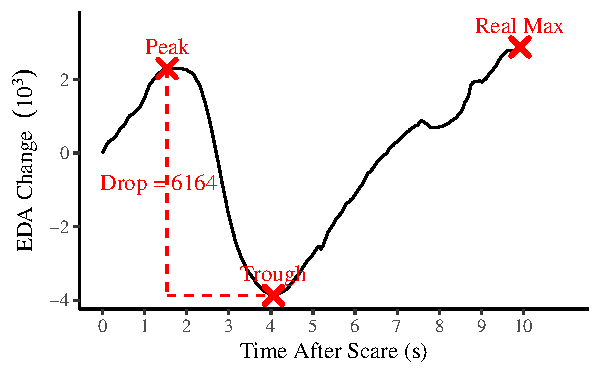
\includegraphics[width=\maxwidth]{figure/ExampleScare-1} 

}



	\caption{How drop size is calculated}
	\label{fig:ExampleScare}
\end{wrapfigure}

The effectiveness of a jump scare is measured in terms of its \emph{drop}, where a large drop indicates a more successful scare.
This is calculated by examining the EDA data for 10 seconds after the scare.
The drop is the difference between the minimum EDA value seen (the \emph{trough}) and the maximum EDA value seen before the minimum (the \emph{peak}).
This is distinct from the real maximum, as we ignore any values after the trough (See \vref{fig:ExampleScare}).

\vspace{20pt}

\begin{minipage}{\textwidth}
\begin{tcolorbox}[colback=black!10, title=Procedure, sharp corners]
	
	\begin{enumerate}
		\item 10 seconds after each scare, compute its drop, appending to a list of drops
		\item If in the calibration phase, stop now
		\item Calculate the mean and standard deviation of the drop list, excluding the last scare
		\item Compute the delay factor:
		
		\begin{figure}[H]
			\centering
			\begin{subfigure}[t]{.45\textwidth}
				\begin{minipage}{\linewidth}
					\begin{equation}
					e^{-0.366 * \frac{d - \mu}{\sigma}}
					\end{equation}
					
					where:
					
					$d$ is the most recent drop
					
					$\mu$ is the mean of previous drops
					
					$\sigma$ is the std. dev. of previous drops
					
					The delay factor is clamped to values between $\frac{1}{3}$ and $3$, to prevent anomalies causing huge changes.
				\end{minipage}
				\caption{Defined Mathematically}
			\end{subfigure}
			\begin{subfigure}[t]{.45\textwidth}
				\begin{minipage}{\linewidth}


{\centering 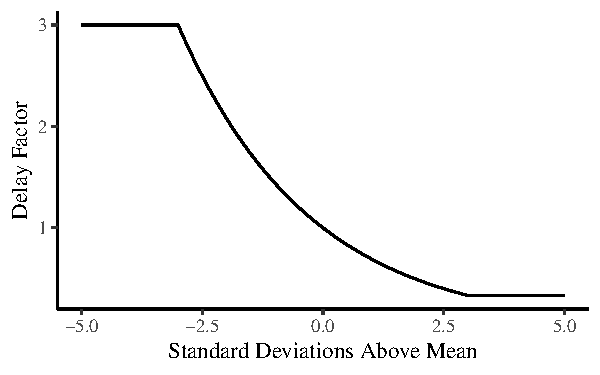
\includegraphics[width=\maxwidth]{figure/DelayFactor-1} 

}



				\end{minipage}
				\caption{Visual Representation}
			\end{subfigure}
		\end{figure}
		
		\item Multiply the delay by the factor
	\end{enumerate}
\end{tcolorbox}
\end{minipage}

\subsection{Control Algorithm}
The control algorithm simply receives a list of scares times as a parameter and scares the user whenever the current time is equal to one of the times in the list.
Determining the values to pass is outside the scope of this algorithm.

\begin{wrapfigure}{r}{0.35\linewidth}
	\vspace{-10pt}
	\centering
	\begin{tikzpicture}
	\draw  [thick](-0.5,0.5) rectangle (-3,-0.5);
	\node at (-1.75,0) {Arduino Uno};
	\node (v6) at (-1.75,0.5) {};
	\node at (-1.75,1.5) {EDA Sensor};
	\draw  [thick](-3.5,-1.5) rectangle (0,-5.5);
	\node (v8) at (-3,0) {};
	\node (v7) at (-3.5,-2) {};
	\node (v4) at (-5,0) {};
	\node (v5) at (-5,-2) {};
	\draw  (v4) edge (v5);
	\draw  [->] (v5) edge (v7);
	\draw  (v8) edge (v4);
	\node at (-4,0.25) {USB Cable};
	\draw  (-3.5,-1.5) rectangle (0,-2.5);
	\node at (-1.75,-2) {jrxtx};
	\node at (-1.75,-1.25) {Minecraft\textit{}};
	\node (v9) at (-1.75,-5) {Delay};
	\node (v10) at (-2.75,-3.5) {Scare};
	\node (v11) at (-0.75,-3.5) {Adjust};
	\node (v12) at (-2.75,-2.5) {};
	\node (v13) at (-0.75,-2.5) {};
	%\draw [->] (v10) edge (v12);
	\draw [->] (v13) edge (v11);
	\draw [->] (v11) edge (v9);
	\draw [->] (v9) edge (v10);
	\draw [->] (v10) edge (v11);
	\node at (-4.25,-1.75) {Serial};
	\draw [->] (-1.75,1.5) node (v1) {} circle (0.5);
	\draw [->] (v1) edge (v6);
	\end{tikzpicture}
	\caption{Game Architecture}
	\label{fig:Architecture}
	\vspace{-10pt}
\end{wrapfigure}

\subsection{Implementation}

\vref{fig:Architecture} shows the hardware and software architecture of the game that was implemented.
An Arduino Uno was used to read from the EDA sensor.
To reduce the noise in the data and the volume of data recorded, it takes 10 readings and sums them, then reports the sum value.
This maintains a sufficiently high data rate, producing one reading every 5--10 ms.
The Arduino operates in an infinite loop, sending readings to the computer using serial over USB.

The horror game was created as a mod for the game Minecraft.
This simplified the process of creating the game, using Minecraft as a base and its mature open-source modding API, Forge, to implement custom functionality.

The first three scares of each playtest are used as the calibration phase.
These first scares happen randomly, 20--30 seconds apart.
The delay produced by the algorithm was clamped to between 0 and 100 seconds.
This was done to maintain a sufficiently high scare rate and increase the amount of data available, and might not be necessary if the algorithm was implemented in a real game.
The delay is not calculated until 10 seconds after the scare.
The delay cannot begin until this point, which means that in practice, the delay is between scares is between 10 and 110 seconds.

When designing the game, there was concern surrounding the difficulty of scaring users enough that their shock would produce a measurable response.
However, the sensor is incredibly sensitive --- even when the user was expecting it, a screen with the word `boo' written on it was enough to get a recognisable response.
This meant that it was trivial to design a scare which generated a suitably large effect that could easily be measured and analysed.

\begin{wrapfigure}{r}{0.4\linewidth}
	\vspace{-10pt}
	\centering
	
\includegraphics[width=\linewidth]{images/scare.png}
	\caption{The Jump Scare}
	\label{fig:JumpScare}
	\vspace{-15pt}
\end{wrapfigure}

The final jump scare is shown in \vref{fig:JumpScare}.
A `creeper' face appears large on the screen.
The creeper is a monster in Minecraft and has a reasonably scary appearance.
At the same time, a loud noise plays consisting of many in-game noises pitch-shifted and played simultaneously.\footnote{A video of the jump scare, with sound, is available at \url{https://www.youtube.com/watch?v=kKKoTZelk3k}}
It has many low frequencies and some high-pitched scream-like sounds, which can help evoke a sense of fear.

The jump scare poses no threat to the player in-game, as any non-random threat must be affected by the game environment.
Since the only knowledge used by the algorithm is previous scare data, it will never time scares well if doing so requires knowledge of the game environment.

Players were asked to explore a haunted house for 10 minutes while spooky music played, searching for 16 coloured wool in hidden chests.
The game environment and music were identical in all playtests (see \vref{fig:GameEnvironment}), with the environment automatically restored from a backup before each test.
The challenge of finding wool ensured that participants continued to explore the house throughout their playtest.
After 10 minutes, the players were automatically informed that the game was complete.
At that point, the jump scares stopped and the data was saved.

\begin{figure}[htb]
	\centering
	\begin{subfigure}[t]{.495\linewidth}
		\centering
		
\includegraphics[width=\textwidth]{images/environment1.png}
	\end{subfigure}
	\begin{subfigure}[t]{.495\linewidth}
		\centering
		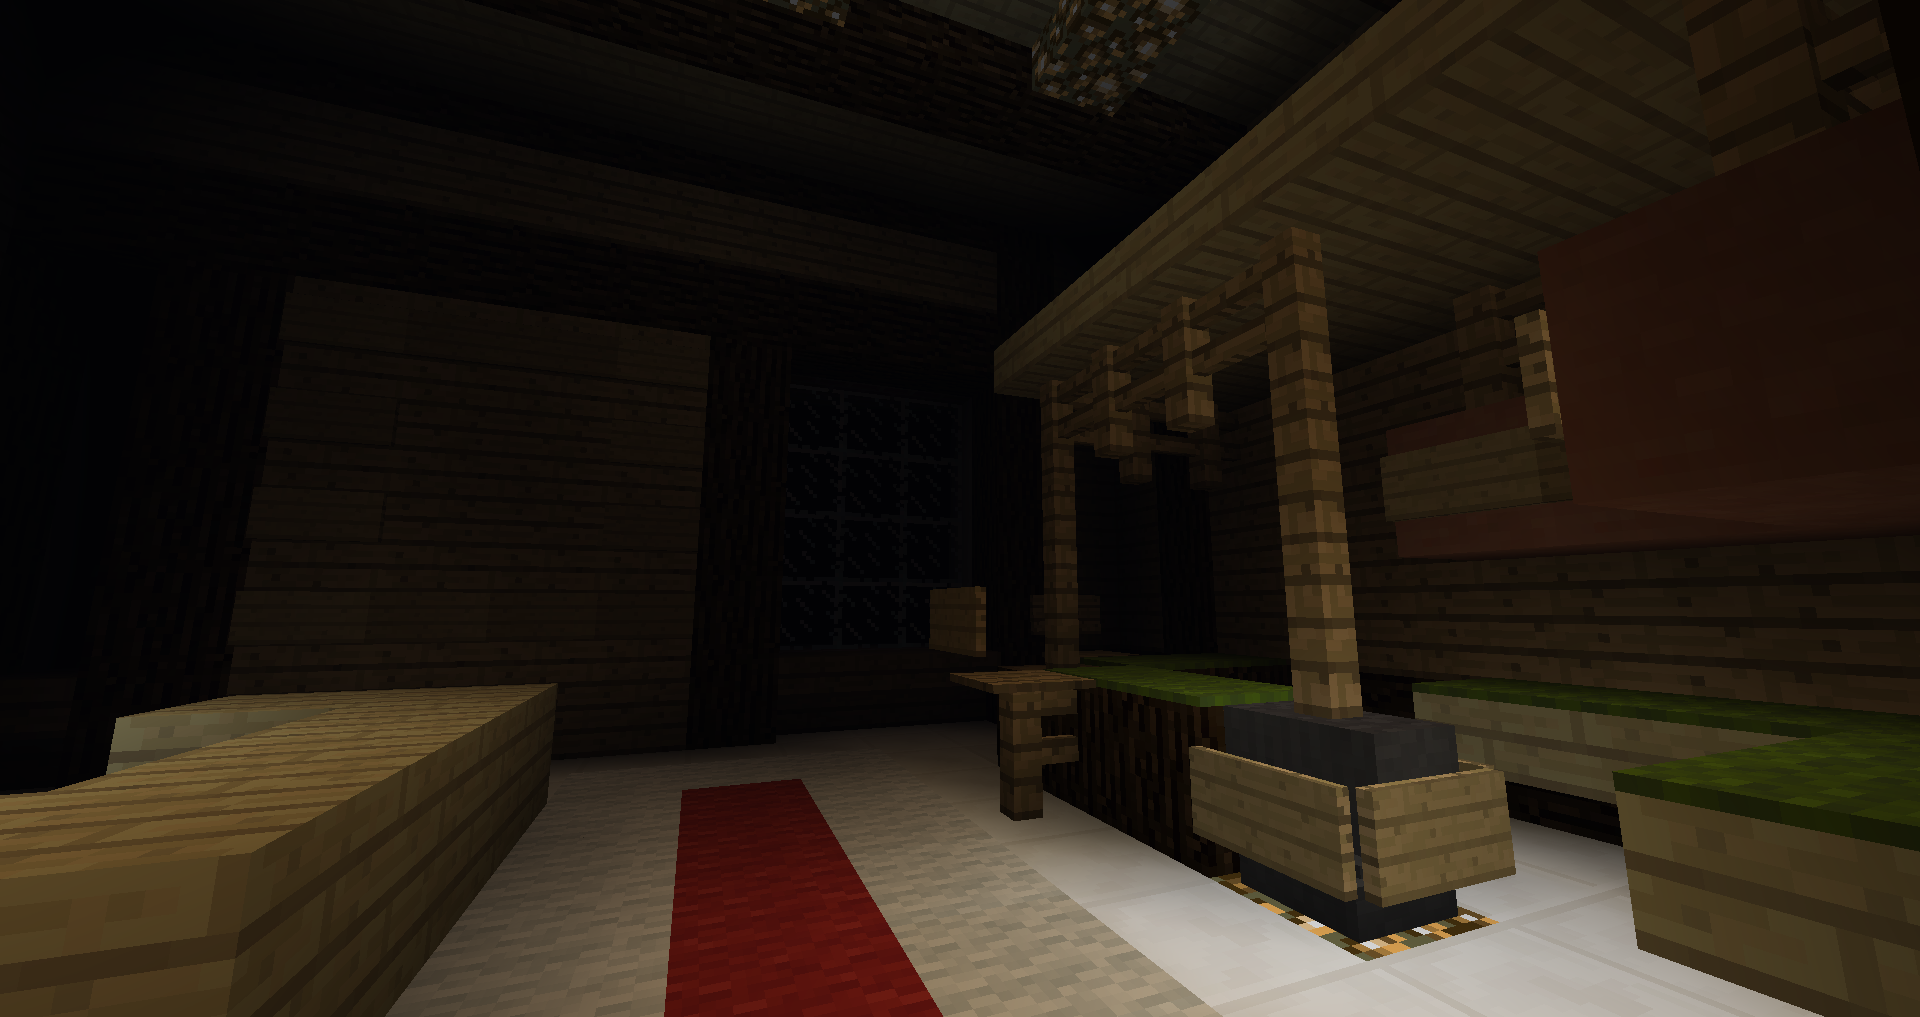
\includegraphics[width=\textwidth]{images/environment2.png}
	\end{subfigure}
	\begin{subfigure}[t]{.495\linewidth}
		\centering
		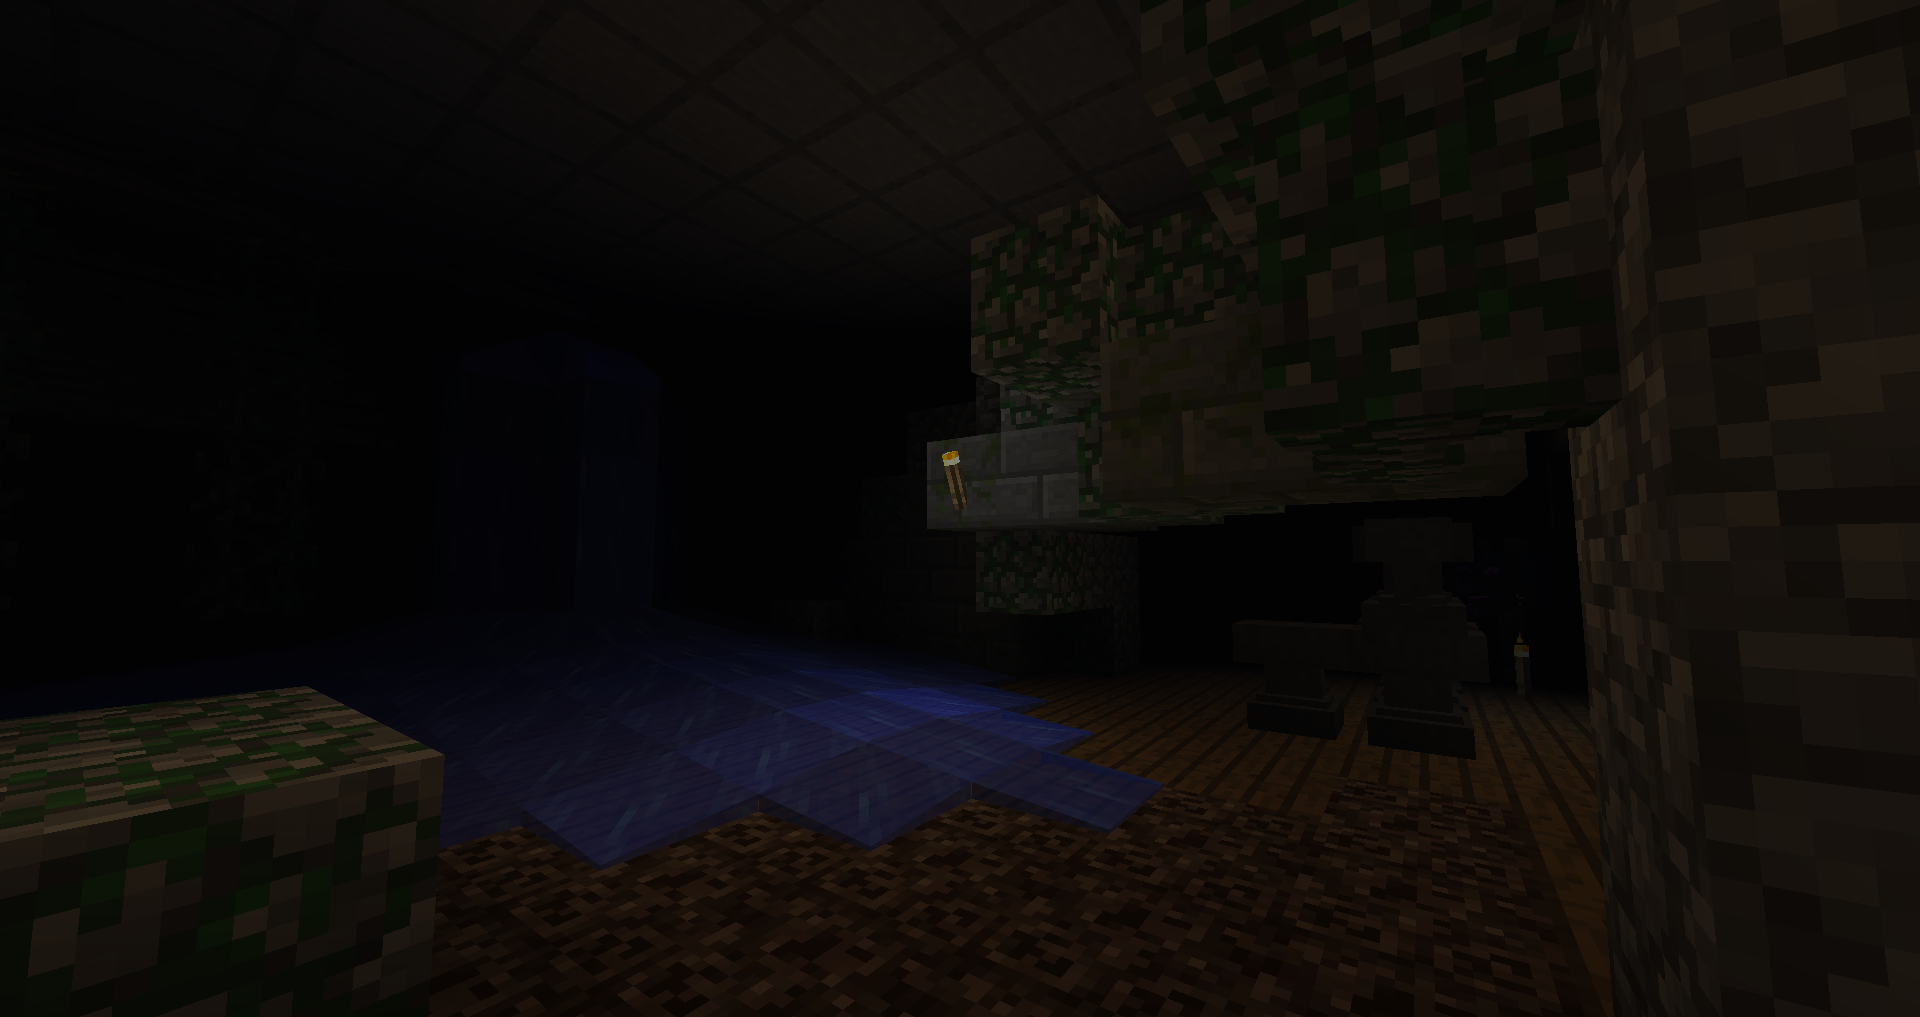
\includegraphics[width=\textwidth]{images/environment3.png}
	\end{subfigure}
	\begin{subfigure}[t]{.495\linewidth}
		\centering
		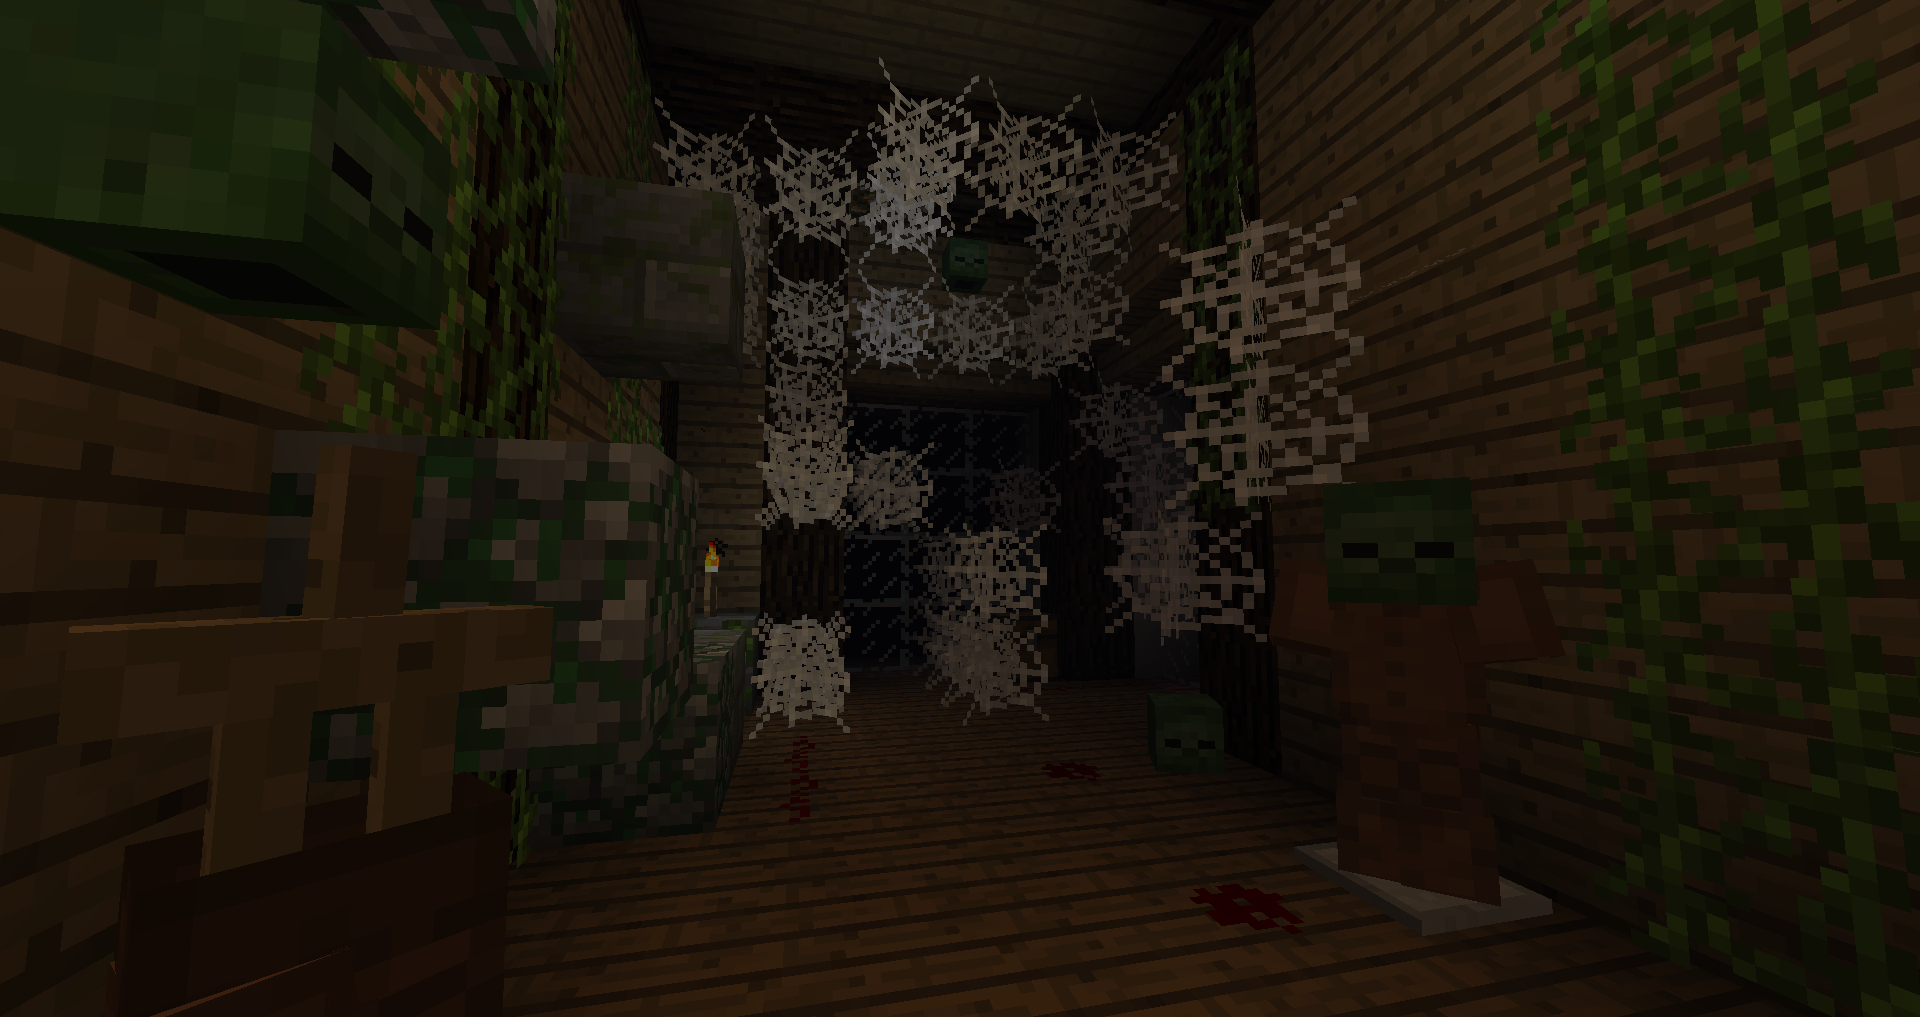
\includegraphics[width=\textwidth]{images/environment4.png}
	\end{subfigure}
	\caption{Examples of the Game Environment}
	\label{fig:GameEnvironment}
\end{figure}


Data from the sensor is recorded for the whole test, allowing more flexibility during analysis.
Playtest start and end times are recorded, in addition to the exact timings of the scares.
When the test ends, all data is saved to a JSON file.
These JSON files are used in the control algorithm for the control group, which simply replicates the scare timings from the data file provided.

\subsection{Software Engineering Design}
Minecraft and Forge are written in Java, meaning that the choice of language was limited to those able to compile to JVM bytecode.
Of the many options, the language Kotlin was chosen for the game.
Compared with Java, it is much more expressive and pragmatic, reducing the amount of boilerplate code that must be written to solve a problem.
Kotlin reduces the incidence of common bugs such as null-pointer exceptions by employing nullable types and improving support for functional programming, which was used throughout the game when handling lists and collections.

The Forge modding API abstracts from the real-time nature of games to an event-based architecture.
The implemented game maintains this style throughout.
Each game tick, which equates to 20 times per second, Forge runs the code provided to it.
We will now explore the main aspects of that code.

\subsubsection{Serial Code}
The Serial code is encapsulated in a separate class.
The Serial code uses the \emph{jrxtx} serial library, which is programmed via pluggable event handlers.
The Serial class attaches its event handler to the library.
This means that every time the library triggers a Serial Event, the Serial class retrieves the serial value and current time, adding them to a large buffer.
The Serial class contains a method to retrieve the last $x$ seconds of data, which is used extensively throughout the rest of the game to reduce code duplication.

\subsubsection{Storytellers}
The game is implemented such that it has two interchangeable \emph{storytellers}.
These filter the game tick events and determine which ones should trigger a jump scare.
There is one storyteller for the dynamic algorithm and one for the control algorithm.

The dynamic storyteller maintains a variable which stores the time of the next jump scare and the current delay between scares.
Each tick, it checks whether the current time is after the time stored in the variable.
If so, it triggers the jump scare and nullifies that variable, setting a timer for 10 seconds.
When the timer event triggers, it accesses the last 10 seconds of data from the serial buffer.
Using that data, the delay factor is calculated and the delay updated, in addition to the variable storing the time of the next scare.
From here, the process repeats.

In comparison, the control storyteller simply loads a data file outputted during a previous playtest.
The scare times are extracted from the data file and loaded into a queue.
Each tick, the storyteller checks whether the current time is greater than the time at the front of the queue.
If so, it gets dequeued and triggers a scare.
No timer is set since no analysis occurs.

Both storytellers extend from a base storyteller superclass which terminates the playtest after 10 minutes, displaying \emph{Test Complete} on the screen.
This triggers the data export, which serialises the data to JSON.

\subsubsection{Development Process}
The development of the game mostly followed a waterfall development philosophy, with some agile elements.
Programs that are used in experiments are distinct from most software projects, as the software cannot be changed or updated in any meaningful way once the experiment has began, to preserve the internal validity of the experiment.
Therefore, any iterative processes must stop before the `client' sees the project for the first time.
However, elements of the agile process were used during the design phase, including repeatedly creating prototype systems and incrementally improving them.
Once the specification for the final algorithm and game was decided, there was no additional user feedback before the experiment began.
This hybrid approach to software development was the most appropriate for this project, as it allowed flexibility when there were many unknowns, and allowed a fixed game to be used once the experiment began.
A more agile process could have been used, and would have been beneficial, but would have meant running multiple pre-tests, using up participants who could have instead participated in the final experiment.
This would have been ideal, but was infeasible given the limited time and resources available.

In total, the game created for the experiment comprises 949 lines of code across 21 classes.

\section{Experimental Study}

This section will discuss the user study that was conducted.
Its null hypothesis was: \emph{There is no difference in user experience when using the dynamic algorithm compared to the control algorithm}.
The alternative hypothesis was simply that there is a difference between the two algorithms.

Participants were put into one of two groups:
\begin{enumerate}
	\item The intervention group (I-group) played the game with the dynamic algorithm running
	\item The control group (C-group) played the game with the control algorithm
\end{enumerate}

In addition to the environment, music, and scares being controlled, many other experimental controls were put in place to improve the reliability of the experimental study.

\begin{wrapfigure}{r}{0.5\linewidth}
	\vspace{-10pt}


{\centering 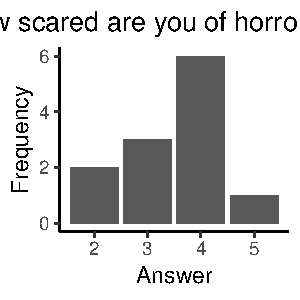
\includegraphics[width=\maxwidth]{figure/ParticipantScaredness-1} 

}



	\caption{Distribution of self-reported fear}
	\label{fig:ParticipantScaredness}
\end{wrapfigure}

\subsection{Controlling for Reported Fear}

We expect that participants who are more scared of the horror genre will have stronger reactions to the jump scare.
Participant pairings were created such that both participants in a pair self-reported the same level of fear for horror games.
One participant in the pair was assigned to the I-group, and the other to the C-group.
This is known as stratified sampling \citep[p. 178]{stratification}, and means that the distribution in self-reported fear between the two groups is identical (see \vref{fig:ParticipantScaredness}).
This stratified sampling controls for participants' self-reported fear, preventing one group from containing more stoic participants than the other, which would have skewed the results.

\begin{wrapfigure}{r}{0.5\linewidth}
	\vspace{-10pt}


{\centering 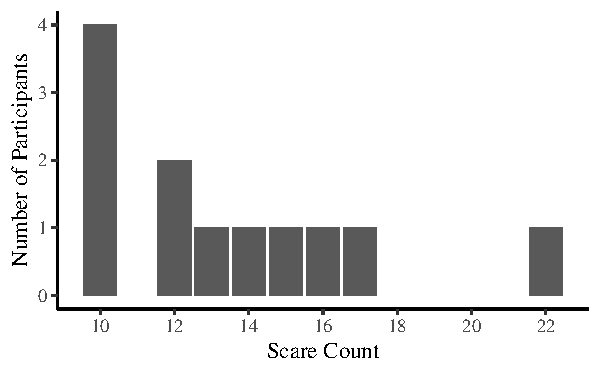
\includegraphics[width=\maxwidth]{figure/ParticipantScares-1} 

}



	\caption{Distribution of scare frequency}
	\label{fig:ParticipantScares}
\end{wrapfigure}


\subsection{Controlling for Scare Frequency}

We also expect participants that are shown more jump scares to become more desensitised.
To control for this, each pairing made previously was shown the same number of scares.
Since the dynamic algorithm cannot target a certain number of scares, the I-group participants of each pair were tested first.
When the C-group participants were tested, each person was shown the same number of scares as their partner.
This means that each group has the same distribution of scare frequencies (see \vref{fig:ParticipantScares}).

\subsection{Controlling for Scare Pacing}

We hypothesise that the timing of a scare affects the strength of the user's reaction.
A number of strategies were considered when creating the control algorithm.
Originally, the scares were going to be spread evenly across the playtest, but that meant that participants learned to expect a scare, which unfairly biased the results against the control algorithm.
This belies that a set of scare timings have an inherent `quality' to them, unrelated to whether the scares were tailored to an individual.
To ensure that this underlying `quality' of timing was the same between the two groups, each C-group participant was scared at the exact same times as their I-group partner.

The study originally aimed to test 50 participants.
Due to time limitations and difficulty accessing participants, only 26 were tested.
Of those, two participants were excluded from analysis as their EDA went below zero and the sensor stopped working, corrupting the data.
Of the remaining 24 participants, 12 were allocated to each group.
After 21 participants had been tested, access to participants decreased due to university vacations, meaning that finding additional participants would become impossible.
From this point, participation was limited to only those who could complete a pre-existing pair.
Prospective participants were not told what answer was needed on the self-reported fear question in order to be approved to participate.

\subsection{Ethics}
Ethical approval was granted in accordance with Durham University Computer Science Department ethical guidelines.
The project was deemed low-risk and did not require approval from the ethics committee.
Participants signed an informed consent form which explained what the study entailed and the experimental setting.
Psychological harm was prevented by allowing participants to ask questions, see the jump scare prior to testing, and drop out freely.
Physical harm was unlikely enough that no special considerations were necessary.
Confidentiality was achieved through the use of participant IDs and only linking ID to name in the consent forms, which were securely destroyed after the experiment was complete.
Data was stored on a password-protected device and has since been released into the public domain as all participants signed a voluntary data release.

\subsection{Threats to Validity}
\label{sec:Validity}
We must acknowledge potential threats and biases that may arise during experimentation.
A threat to validity occurs when the conditions of an experiment are imperfect in such a way that the results could be attributable to alternative causes.
The threats to the validity of the study will be analysed using the framework described in \citet[pp. 5--6]{validity}.

\subsubsection{Internal Validity}
The internal validity concerns whether the experiment is successfully measuring the effect that it aims to measure. Some factors affecting interval validity will be discussed:

\textbf{Maturation} --- When the measured variable is a function of time and there is a time difference between the testing of the two groups.
In each pair, the I-group test happens before the C-group test.
However, the dependent variable is unlikely to be a function of time --- people are not more or less scared of horror games from one week to the next, and there were no newsworthy events to cause heightened fear.

\textbf{Testing} --- When participants take multiple tests and the first test affects future tests.
Retesting would have led to much faster desensitisation, which is one of our main dependent variables.
Therefore this had to be controlled for by having each participant only do a playtest once.

\textbf{Attrition} --- When the risk of people dropping out / being excluded is a function of the dependent variable.
This risk is present in two ways.
If a participant is very scared, they will be more likely to drop out.
Participants who complete the test will therefore be biased towards those who found the scares ineffective, minimising any difference between the groups.
This risk had no impact as nobody dropped out once starting the playtest.

Two participants were excluded because their skin resistance was so low that the sensor broke.
At first, this appears like a serious attrition risk.
However, the low skin resistance was not due to a large drop, but due to their naturally low baseline.
This means that the attrition was caused by factors unrelated to the experiment, and attrition threats are minimal.

\textbf{Selection of Subjects} --- When the two groups have different characteristics which affect the dependent variable.
Much of this was controlled for by using stratified sampling, where we controlled for self-reported fear.
Since the I-group participant in each pair was found first, they will be closer friends with the researcher, as participants were selected based on availability.
This threat could be reduced by sampling participants randomly, getting an initial expression of interest and a self-reported fear rating, then assigning groups and performing tests.
This was planned originally, but found to be infeasible due to the increased attrition rates of having a two-phase sampling strategy.

\begin{wrapfigure}{r}{0.5\linewidth}
	\vspace{-25pt}


{\centering 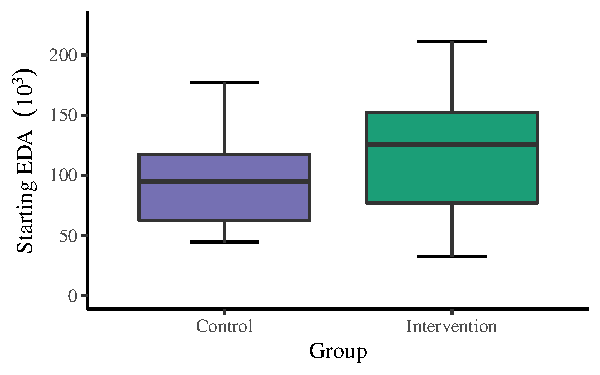
\includegraphics[width=\maxwidth]{figure/StartingEda-1} 

}



	\caption{Initial EDA per group}
	\label{fig:StartingEda}
\end{wrapfigure}

Additionally, participants begin the playtest with different EDA levels, and on average the starting EDA of the two groups differs (see \vref{fig:StartingEda}).
As higher EDA leads to larger drops as a result of the same stimulus, this makes it harder to compare between the groups.
This threat is one of the project's most significant threats.

\textbf{Environmental} --- When the test environment differs between participants.
Some tests were performed in a university computer science department, which contains many distractions, while other tests were performed in quiet, private areas.
Some tests were performed at social events, meaning that participants had been drinking alcohol, though no participant was noticeably drunk.
These factors were not recorded and therefore it is impossible to investigate any correlation between the environmental factors and results.

\begin{wrapfigure}{r}{0.5\linewidth}
\vspace{-15pt}


{\centering 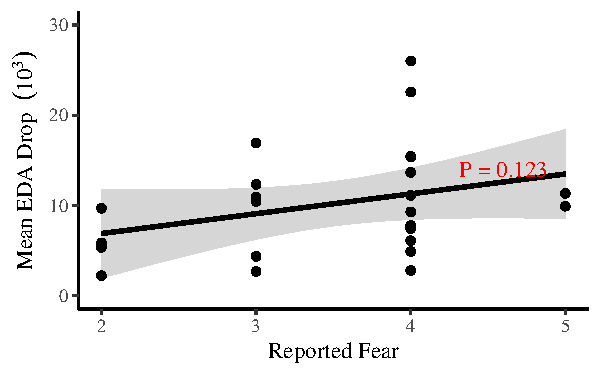
\includegraphics[width=\maxwidth]{figure/ReportedScaredness-1} 

}



	\caption{Predicted vs Actual Fear}
	\label{fig:ReportedScaredness}
\end{wrapfigure}

\textbf{Data Vandalism} --- When the data is intentionally corrupted by the participants.
There is a slim chance of intentional data vandalism.
Participants could lie on self-reported fear, but \vref{fig:ReportedScaredness} shows no clear evidence of lying.
The data generally follows the regression line, but with a wide variance --- this suggests that the participants are truthful but inaccurate.
Participants could intentionally change their EDA, but this requires training and is a very niche skill, meaning it can be ruled out as a possibility.

\subsubsection{External Validity}
The external validity concerns whether the experiment is generalisable to the population.
Two factors impacted the external validity of the user study.

\textbf{Interaction effects of selection biases and the experimental variable} --- When the sample is not representative of the population and reacts differently.
The majority of participants were young, male, and many of them were computer scientists.
It is not clear whether these participants would react to the intervention differently than the population.
Therefore, it is impossible to rule out this threat.

\textbf{Not generalisable to realistic gameplay} --- When the experimental arrangements are different to the real-world use of the intervention.
It is not clear whether a 10-minute test would generalise to a multi-hour play session, but limiting the test length was necessary for practical reasons.
Additionally, it's not clear whether a simple game based in Minecraft where all jump scares are the same would generalise to a more complex game, with multiple kinds of jump scare.
Limiting the test to a simple game was necessary in this first experiment to control for as many factors as possible, but means that additional tests with more complex games will be necessary before we can be confident that the data is generalisable to real-world use.

\section{Results}

This section will state the results from the user study and provide visualisations of the data.
We will first discuss the data recorded from the EDA sensor, before moving on to examine the results of the questions asked to participants after their playtest was completed.

\subsection{Empirical Data}
For context, the raw data from the sensor is shown in \vref{fig:RawData}.
The data shown has already been normalised from \emph{wallclock time} to \emph{time after playtest start}.

This data evidently required significant cleanup before it was ready to be analysed.
The decision was made to record all data in full, rather than pre-emptively deciding to only record some of the EDA data.
This came at the expense of additional storage space and computation time, but meant that no analysis decisions were made pre-emptively.

\vref{fig:PerGroupScares} shows the data after being filtered to the 10 seconds after each scare and lines ar coloured based on the participant's group.
Lines with a larger vertical drop generally indicate a stronger reaction to a scare.

\begin{figure}[htb]
	\centering
	\begin{subfigure}[t]{.49\linewidth}


{\centering 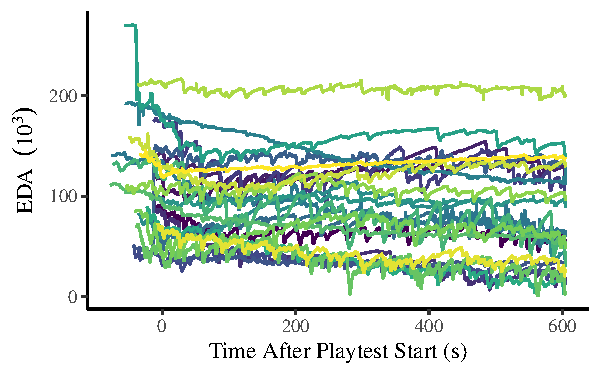
\includegraphics[width=\maxwidth]{figure/RawData-1} 

}



		\caption{Raw data from the sensor}
		\label{fig:RawData}
	\end{subfigure}
	\begin{subfigure}[t]{.49\linewidth}


{\centering 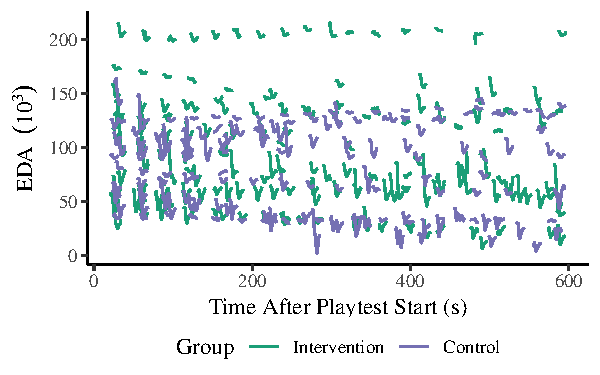
\includegraphics[width=\maxwidth]{figure/PerGroupScares-1} 

}



		\caption{Scare data, coloured per group}
		\label{fig:PerGroupScares}
	\end{subfigure}
	\caption{Data pre-analysis}
	\label{fig:Data}
\end{figure}

By normalising all of these scares to start at $(0,0)$, and taking the mean of each group's lines, we can see each group's average scare.
We can also calculate a standard error margin around these means.
When doing so, we filter out the calibration scares.
The average scare of the two groups differs significantly, with participants in the I-group seeing their EDA fall for longer and to a lower trough value (see \vref{fig:ResponseAfterScare}).
The I-group also takes longer to recover, with the two lines still being separated by more than the margin of error after 10 seconds.
Additionally, the I-group reacts slightly quicker than the C-group, with the EDA starting to drop slightly earlier than it does for the C-group.
The same trend can be seen in \vref{fig:ResponseAfterScareRel}, which controls for starting EDA by plotting a relative drop instead of an absolute drop.

\begin{figure}[htb]
  \centering
  \begin{subfigure}[t]{.49\linewidth}


{\centering 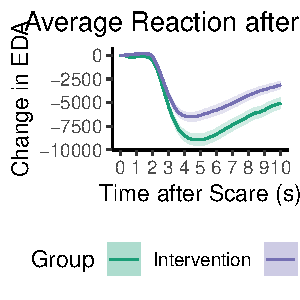
\includegraphics[width=\maxwidth]{figure/ResponseAfterScare-1} 

}



    \caption{Per-Group Average}
  \end{subfigure}
  \begin{subfigure}[t]{.49\linewidth}


{\centering 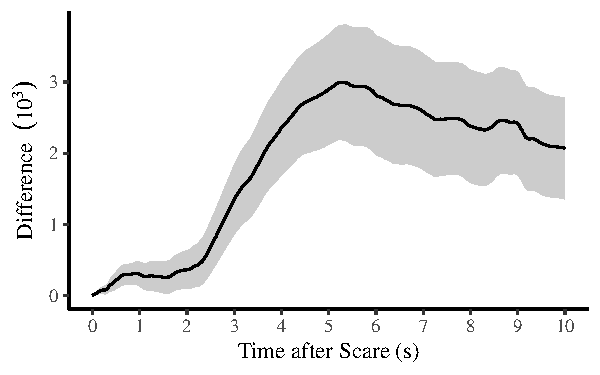
\includegraphics[width=\maxwidth]{figure/CompareGroups-1} 

}



    \caption{Difference between Groups}
  \end{subfigure}
  \caption{Average Response to a Jump Scare}
  \label{fig:ResponseAfterScare}
\end{figure}

\begin{figure}[htb]
	\centering
	\begin{subfigure}[t]{.49\linewidth}


{\centering 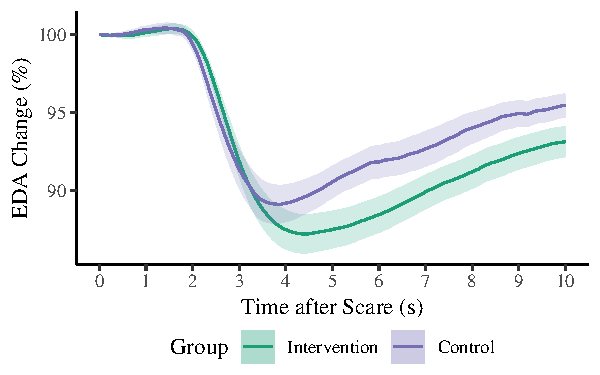
\includegraphics[width=\maxwidth]{figure/ResponseAfterScareRel-1} 

}



		\caption{Per-Group Average}
	\end{subfigure}
	\begin{subfigure}[t]{.49\linewidth}


{\centering 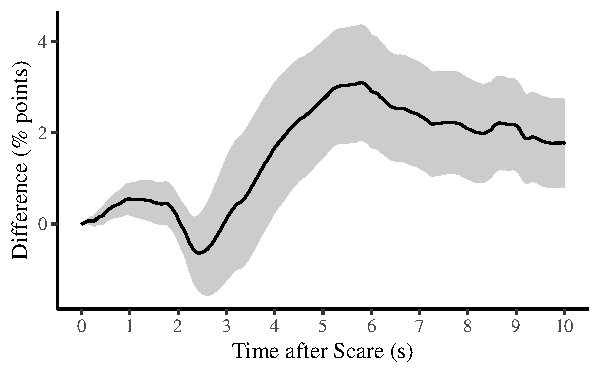
\includegraphics[width=\maxwidth]{figure/CompareGroupsRel-1} 

}



		\caption{Difference between Groups}
	\end{subfigure}
	\caption{Average Relative Response to a Jump Scare}
	\label{fig:ResponseAfterScareRel}
\end{figure}

If we take the data from \vref{fig:PerGroupScares}, and convert each scare line to its calculated drop value, we can plot how the size of the drop changes over time.
\vref{fig:ScarednessOverTime} shows every scare that occurred during the experiments, and plots one linear regression per group.
At the time of the first scares, the linear regressions predict almost exactly the same drop size for both groups.
This is a strong indication that the sample is valid and that the two groups begin with the same reactions before the algorithm has kicked in.
As time goes on, the linear regressions diverge, separating by more than a 95\% confidence interval by the mid-way point of the playtest.
This indicates that the dynamic algorithm prevents the I-group from desensitised to the jump scares.

\begin{figure}[htb]
	\centering
	\begin{subfigure}[t]{.49\linewidth}


{\centering 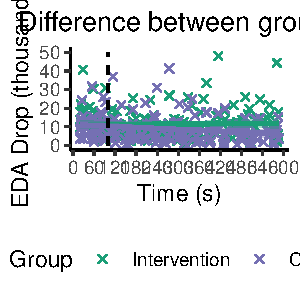
\includegraphics[width=\maxwidth]{figure/ScarednessOverTime-1} 

}



		\caption{All data}
	\end{subfigure}
	\begin{subfigure}[t]{.49\linewidth}


{\centering 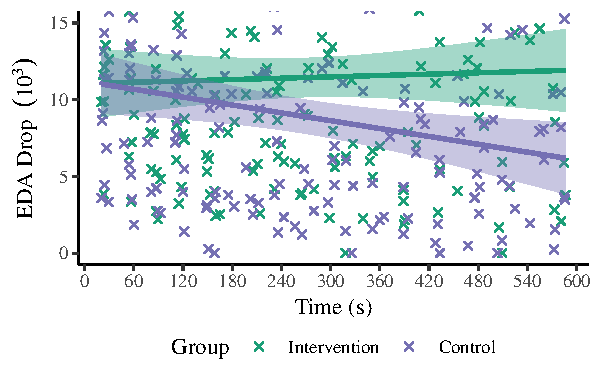
\includegraphics[width=\maxwidth]{figure/ScarednessOverTimeCrop-1} 

}



		\caption{Zoomed to show trends}
	\end{subfigure}
	\caption{Scaredness over Time}
	\label{fig:ScarednessOverTime}
\end{figure}

\begin{wraptable}{r}{0.5\linewidth}
	\vspace{-20pt}
    \caption{Regression Statistics}
    \label{tab:RegressionTable}
	\vspace{-20pt}
    \begin{footnotesize}
    	\begin{center}

\begin{tabular}{cccc}
\toprule
\textbf{Model} & \textbf{Gradient} & \textbf{R-Squared} & \textbf{P-Value}\\
\midrule
Intervention & 1.47 & 0.001 & 0.695\\
Control & -8.54 & 0.042 & 0.009\\
\bottomrule
\end{tabular}

		\end{center}
	\end{footnotesize}
	\vspace{-20pt}
\end{wraptable}

\vref{tab:RegressionTable} shows the relevant statistics of the two regressions.
The P-Value of the C-group is under 0.01, and its gradient is negative, indicating a statistically significant trend.
Over time, the C-group becomes less scared of the jump scares.
The R-Squared value indicates that around 4\% of a control-group participant's response to a scare can be predicted solely by how long they have been playing.
The gradient indicates that for each second played, a participant in the C-group would respond to a scare with a drop that is 8.5 points smaller.

In comparison, the P-Value of the I-group is above 50\%, indicating that it's likely there is no correlation between time played and scaredness in the I-group.
Even if there was a correlation, the gradient is positive indicating that participants actually become more scared over time.

\subsection{User Self-Reported Measures}
\begin{wrapfigure}{r}{0.5\linewidth}
	\vspace{-30pt}


{\centering 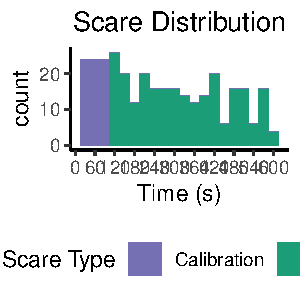
\includegraphics[width=\maxwidth]{figure/ScareHistogram-1} 

}



	\caption{Scare Frequency over Time}
	\label{fig:ScareHistogram}
\end{wrapfigure}

Participants were asked how much they enjoyed the game (see \vref{fig:ParticipantEnjoyment}).
In general, participants in the I-group enjoyed the game slightly less than those in the C-group.

\begin{figure}[htb]
	\centering
	\begin{subfigure}[t]{.49\linewidth}


{\centering 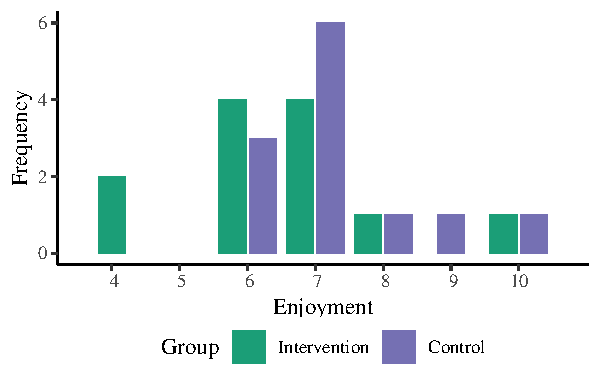
\includegraphics[width=\maxwidth]{figure/ParticipantEnjoyment-1} 

}



		\caption{Distribution of Responses}
	\end{subfigure}
	\begin{subfigure}[t]{.49\linewidth}


{\centering 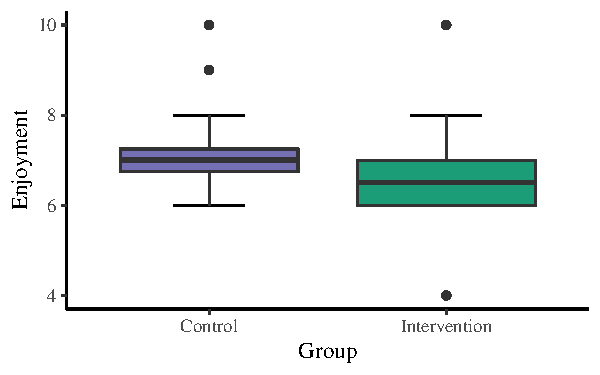
\includegraphics[width=\maxwidth]{figure/ParticipantEnjoymentBoxPlot-1} 

}



		\caption{Comparison between Groups}
	\end{subfigure}
	\caption{On a scale of 1-10, how much did you enjoy that as a game?}
	\label{fig:ParticipantEnjoyment}
\end{figure}

Participants were asked to rate the frequency of the jump scares (see \vref{fig:ParticipantTiming}).
Most participants felt there were too many jump scares.
Their feeling is backed up by the scare timing histogram (see \vref{fig:ScareHistogram}), which shows that the algorithm generally decreased the frequency of jump scares over time.
The C-group felt marginally more strongly that there were too many scares.
This was not the result of a real difference is scare frequency as each group had identical scare timings.
Therefore, this suggests that the scares were badly timed for the C-group, making the scares less immersive.

There is a stastically significant positive correlation between the frequency of jump scares and participants' perceived scare frequency (see \vref{fig:ParticipantTimingRegression}).
This indicates that participants accurately assess the frequency of jump scares.

\begin{figure}[htb]
	\centering
	\begin{subfigure}[t]{.49\linewidth}


{\centering 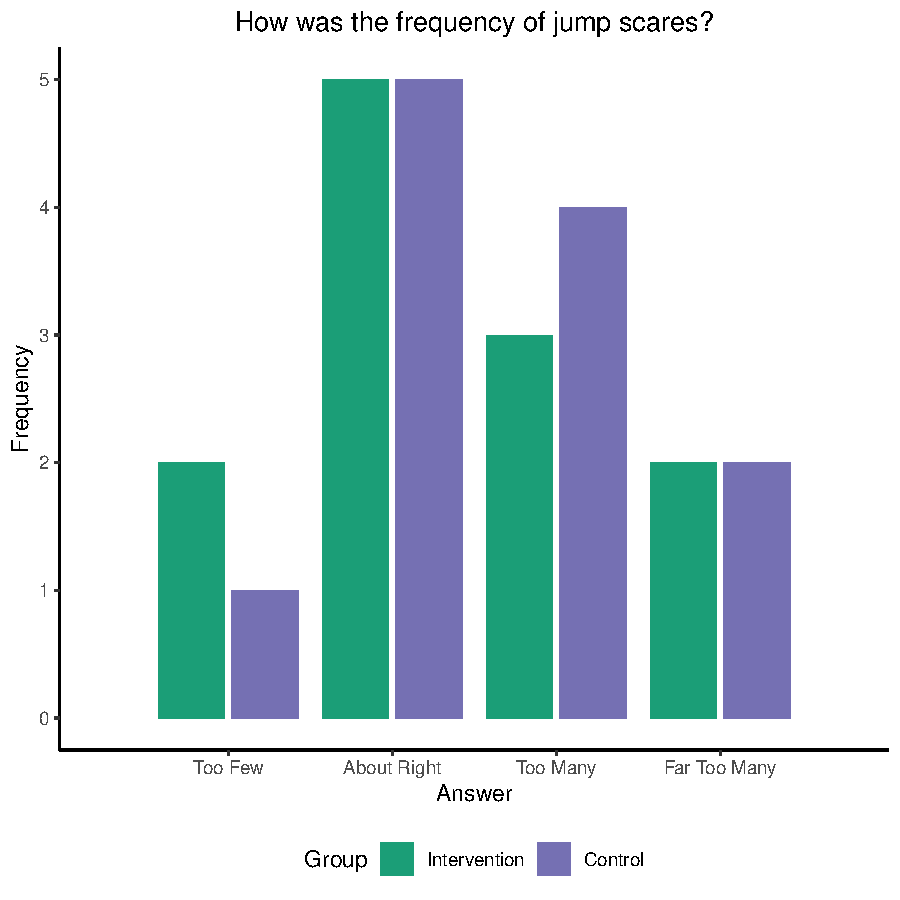
\includegraphics[width=\maxwidth]{figure/ParticipantTiming-1} 

}



		\caption{Distribution of Responses}
	\end{subfigure}
	\begin{subfigure}[t]{.49\linewidth}


{\centering 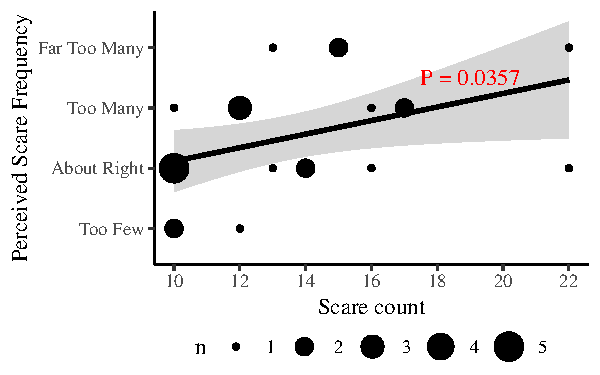
\includegraphics[width=\maxwidth]{figure/ScareFrequency-1} 

}



		\caption{Actual vs Perceived frequency}
		\label{fig:ParticipantTimingRegression}
	\end{subfigure}
	\caption{How was the frequency of jump scares?}
	\label{fig:ParticipantTiming}
\end{figure}

\section{Analysis}
\label{sec:Analysis}

This section will explore the results in terms of their validity and generalisability.
The potential impact on commercial games and further research will be considered.

\subsection{Empirical Data}

The results show that the I-group is, on average, significantly more scared than the C-group (see \vref{fig:ResponseAfterScare}).
They drop further, faster, and for longer.
However, the I-group also starts at a higher EDA, so their drops will naturally be bigger.
Due to the mechanics of EDA, a shock produces sweat which takes time to evaporate before the EDA can recover.
Therefore fact that the I-group and C-group recover at almost the same speed suggests that the data is valid.
The I-group was more scared than the C-group, and this is likely to generalise since the margin was fairly wide and remained when examining both the absolute and relative drop.
A larger study with a bigger sample and tighter control for initial EDA would be better equipped to determine which effects are generalisable.

In \vref{fig:ResponseAfterScareRel}, we instead look at the drop in relative terms.
This completely removes the effect of higher EDA showing larger drops, and biases the data in the opposite direction, since higher initial EDA leads to smaller relative drops.
Interestingly, the two lines now drop at around the same time, and drop at roughly the same speed.
However, the I-group line drops for longer and to a lower trough value.
The two lines are separated by more than the margin of error, indicating that the starting EDA is not the reason for the difference between the groups.
It is likely that the intervention causes the I-group to be more scared by the jump scares.

The result that the I-group did not become desensitised over time while the C-group did (see \vref{fig:ScarednessOverTime}) is the most convincing evidence of the project's success.
The two groups have almost identical reactions during calibration.
In the C-group, there's a strong downwards trend over time, with participants becoming desensitised by the jump scares and not reacting as strongly.
Meanwhile, in the I-group there is no such trend.
More importantly, since we are not comparing the groups to each other but to themselves at an earlier time, the issues of different starting EDA between groups is not relevant.
Although a longer test would be needed to confirm it, this chart strongly suggests that the dynamic algorithm will improve the longevity of a horror game, allowing long play sessions before desensitisation.

\subsection{User Self-Reported Measures}
There is a slight difference in participant enjoyment between groups (see \vref{fig:ParticipantEnjoyment}).
Since the difference is small, it could be random noise caused by the small sample size.
Alternatively, it could be due to biases in the sampling as discussed earlier.
Additionally, only one question about enjoyment was asked in the post-test questionnaire, and no demographic data was recorded, so we can't examine the cause of a difference between groups.
Finally, the participants aren't necessarily the target audience of a horror game, as enjoying horror games wasn't a requirement to participate.
Further study to explore whether the algorithm improves enjoyment in horror-game players would be warranted.
It seems suspect that a (fairly mild) horror game can become more scary but less enjoyable --- intuitively, those should be correlated.
The use of a 10-point scale increases the effect of randomness.

The results show a very marginal difference between groups when it comes to the perceived frequency of jump scares (see \vref{fig:ParticipantTiming}).
A large difference would be unexpected, since participants are rating the same underlying frequencies.
This could be interesting to investigate further, and with a larger sample size we could conclusively say that there is a difference between groups.
\vref{fig:ParticipantTimingRegression} shows that around 10 scares is the ideal number, equating to one scare per minute.
However, the benefit of more data outweighs the downside of slight desensitisation due to too many scares.
The high scare frequency is unlikely to invalidate any of the data.

\section{Conclusions}

This project aimed to answer the research question \emph{Can biosignals be used to tailor the timing of scares in a horror game to improve the user experience?}
An algorithm which controlled the timing of jump scares based on EDA data was implemented.
The algorithm increased scare frequency when the player had an above-average reaction, and decreased scare frequency when the player had a below-average reaction.
This algorithm was integrated into a horror game environment and compared to predetermined timings in a user study.
The user study identified that the dynamic algorithm resulted in scarier gameplay and less desensitisation to the scares.

\subsection{User Study}

The user study compared an intervention group, who played with the dynamic algorithm enabled, and a control group, who played with pre-determined timings.
The study controlled for self-reported fear of horror games, scare frequency, and scare timing.
The scare timings for the control group were determined by copying the timings from a member of the intervention group.
The main weaknesses of this study were its small sample size ($n=24$) and that initial EDA was not controlled for.
Initial EDA was significantly higher in the intervention group, which means that the same scare causes a larger absolute drop and a smaller relative drop in EDA.

The intervention group reported that the game was slightly less enjoyable and that scares were marginally less frequent compared to the control group.
The small sample size and numerous threats to internal validity mean that no conclusions can be made about the intervention's effect on enjoyableness or perceived scare frequency.

The intervention group had a larger reaction on average, whether looking at the absolute or relative change in EDA.
By both measures, the two groups were more than the margin of error apart, suggesting that the algorithm is effective in scaring players more.
Since both absolute and relative drops were larger for the intervention group, this is not simply due to the difference in initial EDA.

Generalising to the population, players who used the dynamic algorithm did not become desensitised over time ($P = 0.695$).
Comparatively, players in the control group became desensitised over time ($P = 0.009$).
Since we are comparing each group to itself, initial EDA has no effect.
We can conclude that the algorithm was successful at preventing scare desensitisation.

The validity of the study's results is questionable, due to a number of environmental factors that were not controlled for.
The user study was conducted across multiple environments, and some participants had been drinking alcohol, which could affect how EDA changed in response to scares.

\subsection{Research Objectives}

Almost all research objectives were successfully completed.
All minimum objectives were completed --- a haunted house environment was created for players to explore, and their EDA was tracked while doing so.
A jump scare event was created which caused a measurable scare reaction in the player.
All intermediate objectives were completed --- an algorithm was created which continuously analyses user data and times scares based on the effectiveness of previous scares.
A control algorithm was created which scared users on a predetermined schedule.
Only the first advanced objective was completed --- a user study was conducted.
The algorithm was not revised based on the user study due to lack of time and infeasibility of gathering a second sample of users who had not already played the game.

\subsection{Project Implications}

Further research into this algorithm and the use of EDA for tailoring horror games is recommended, as this study provides promising preliminary results.
Future research should conduct all tests in a controlled environment without distractions.
Additionally, a larger sample size should be gathered, which will improve the initial EDA distribution.
When gathering the sample, participants should be asked to register interest and self-report their fear of horror games, before being randomly assigned to groups.
This may require an incentive to reduce participant attrition after the initial expression of interest.
Additionally, the research should explore if the algorithm prevents desensitisation over longer periods, as this study only tested each participant for 10 minutes.

Future avenues for research could involve using additional sensors, such as a heart rate sensor.
This would allow the system to sense tension in the user, which could be incorporated into a more complex algorithm which tries to scare users when they are feeling most tense.
Alternatively, future research could extend the algorithm to use multiple kinds of scares, discovering which kind of scare is most effective for a given participant --- for example, a person with arachnophobia would have a larger response to spider-based scares.

This study shows promising results but does not provide enough convincing evidence to recommend incorporating the algorithm into commercial games at this time.
There are too many threats to the validity of the study to be confident that the results are valid, and there is little evidence that the results are generalisable to more complex games with longer play times.
If successfully integrated into a commercial game, this algorithm shows great promise for both developers and players.
For developers, they would no longer need to manually program where each scare should go, as it would automatically be tailored to the player.
For players, they would be able to enjoy a scarier game with improved replayability.

\section{References}
\footnotesize\bibliography{projectpaper}
\end{document}
